\section{Related Models for Work Stealing}
\label{sec:Refer-Model-WS}
\index{PerfModel!Related Models for Work Stealing}

\begin{figure}[t]
  \centering
  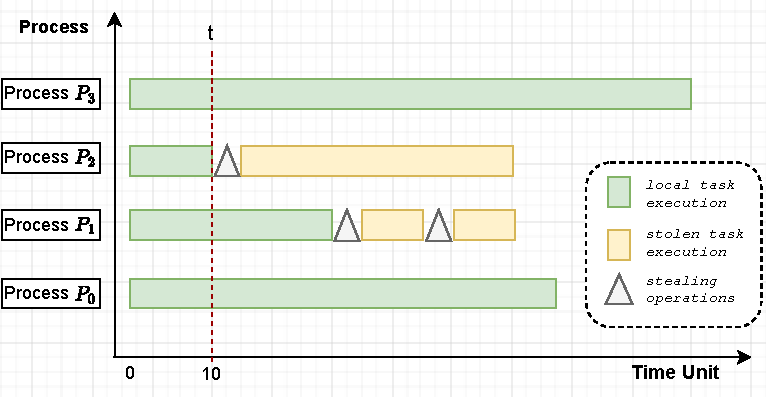
\includegraphics[scale=0.8]{./pictures/perf_analysis_model/perf_analysis_related_model_without_latency.pdf}
	\caption{An illustration of work-stealing without latency concern.}
	\label{fig:perfmodel_relatedmodelwithoutlatency}
\end{figure}

As mentioned, we illustrate again an example of work stealing behaviors in Figure \ref{fig:perfmodel_relatedmodelwithoutlatency}, but this case is without latency concern. This model is commonly known in shared memory systems. The idea is that idle processes will try to steal tasks from other busy processes. Communication is assumed very fast to send and receive tasks immediately. As we can see, the x-axis shows the execution progress by time, along with four processes indexed from 0 to 3. The triangles represent stealing operations at a time. This is an ideal case for load balancing when the time to send and receive tasks is almost instantaneous.\\

To demystify the related models and our proposed model in the next sections, we attempt to merge some related terminologies as well as notations so that they are consistent in this thesis. For example, the total number of tasks is reused and named $T$, distributed on $P$ processes before execution. Table \ref{tab:mapped_notation_table} will show in detail the other related notations. Such the concern, each process in $P$ after a given distribution of $T$ tasks will hold a subset of $T_{i}$ tasks. In some related works, they used $w_{i}$ to indicate the number of tasks at process $i$  \cite{tchiboukdjian2013decentralized}. Thereby, we try to make it consistent with us by using $T_{i}$ as the number of tasks in process $i$. In the following sections, there might be some additional terms about the queue information, and $Q_{i}$ is used to denote the queue status, and they still refer to the values of the number of tasks. Mapping them to the time progress, this may have the field of time $(t)$ following. For instance, $T_{i}(t)$ means the number of tasks in process $i$ at time $t$, or $T(t)$ without $i$ means the total number of tasks (including all processes) at time $t$. The text might re-mention these notations in some specific paragraphs when we want to show further explanation.\\

\begin{table}[t]
\centering
\begin{tabular}{|l|p{2cm}|p{5cm}|p{4.5cm}|}
\hline
\textbf{No.} & \textbf{Notations} & \textbf{Description} & \textbf{Note}        \\ \hline
1  & $T$          & the number of tasks indexed $\left \{0,...,(T-1) \right \}$ & In some other related works, people used $W$ instead of $T$   \\ \hline
2  & $P$					& the number of processes, $\left \{0,...,(P-1) \right \}$    & Other works might use $m$ identical processors instead of $P$ \\ \hline
3  & $T_{i}$			& the set of assigned tasks in Process $i$                    & Other works might use $w_{i}$ instead of $T_{i}$              \\ \hline
4  & $L_{i}$			& the total load of Process $i$                               &                                             \\ \hline
5  & $w_{i}$			& the wallclock execution time of a task, i.e., task $i$      &                                             \\ \hline
6  & $W_{i}$ 			& the wallclock execution time of Process $i$                 &                                             \\ \hline
7  & $S_{P_{i}}$	& processing speed (performance model) of Process $i$         &                                             \\ \hline
8  & $Slow_{i}$		& slowdown coefficient of Process $i$ at runtime              &                                             \\ \hline
9  & $W_{par}$		& the total wallclock execution time (makespan)               & Also called completion time ($C$)           \\ \hline
10 & $R_{imb}$		& imbalance ratio                                             &                                             \\ \hline
11 & $\lambda$		& communication or network latency                            &                                             \\ \hline
12 & $d$					& delay or transmission time                                  &                                             \\ \hline
13 & $B$					& network bandwidth                                           &                                             \\ \hline
14 & $O_{ij}(t)$	& the number of offloaded tasks from Process $i$ to $j$       & The authors in \cite{tchiboukdjian2010tighter} used $R(t)$ as the number of task requests in global after time $t$ \\ \hline
\end{tabular}
\caption{Used notations in the thesis comparing to the notations from related works.}
\label{tab:mapped_notation_table}
\end{table}

The main purpose of performance modeling is to show an upper bound of balancing efficiency with how many tasks can be migrated. Extended from an original work \cite{Blumofe1999OriginWS}, Tchiboukdjian et al. have proposed a good model for work-stealing without latency since 2010 \cite{tchiboukdjian2010tighter} \cite{tchiboukdjian2013decentralized}. In this section, we attempt to summarize their reference models. The first is mentioned as work stealing model without communication latency \cite{tchiboukdjian2010tighter} \cite{tchiboukdjian2013decentralized}. The second is timely analyzed by \cite{gast2021analysis} in 2021, also work stealing but with latency variable.\\

In \cite{tchiboukdjian2013decentralized}, Tchiboukdjian et al. considered a parallel platform with $P$ processes. At time $t$, $T_{i}(t)$ represents the amount of works\footnote{At this point, works are considered as tasks in our context. Therefore, they might be used interchangeably.} on process $i$. Compared to $t=0$, $T_{i}(t)$ will be decreased by time progress. For example, at $t=0$ the workload is just distributed on each process, $T_{i}(t_{0}) = 100$ means holding 100 tasks before running. Then, at $t=10$ assume that 10 tasks have been done on process $i$, and $T_{i}(t_{10})$ would be $90$ such the remaining tasks. We can take Figure \ref{fig:perfmodel_relatedmodelwithoutlatency} as an example, at $t=10$ process $3$ has done 10 tasks and its queue remains 90 tasks, $T_{0}(t_{10}) = 90$. In constract, process $2$ is faster and it has done all tasks at $t=10$, therefore, $T_{2}(t_{10}) = 0$.\\

Therefore, the execution behavior will be simplified as follows,
\begin{itemize}
	\item when $T_{i}(t) > 0$, processor $i$ is active and execute tasks, $T_{i}(t+1) \leq T_{i}(t)$.
	\item when $T_{i}(t) = 0$, processor $i$ is idle and intends to steal tasks from a random processor $j$.
\end{itemize}

\noindent \textbf{A Tight Analysis of Work Stealing \cite{tchiboukdjian2010tighter,tchiboukdjian2013decentralized}}\\

If work stealing is applied, some tasks are moved around, then $T_{i}(t)$ will increase or decrease, depending on how many steal requests and tasks are performed at a time. Tchiboukdjian et al. \cite{tchiboukdjian2010tighter} \cite{tchiboukdjian2013decentralized} assumed that between time $t$ and $t+1$, there are $P - \alpha(t)$ steal requests, $P$ is the total number of processes and $\alpha(t)$ denotes the number of active processes, $\alpha(t) \in [0, m]$. When $\alpha(t)=0$, it means all queues are empty as well as the execution is complete. Corresponding to the sucess steal requests, process $j$ will transfer an amount of work to $i$ and $T_{i}(t+1) + T_{j}(t+1) \leq T_{j}(t)$. Similar to when $\alpha(t)=0$, the execution will terminate if $\forall i \in P, T_{i}(t) = 0$. At time $t$, the total number of tasks on all processes is denoted by $T(t) = \sum_{i=1}^{P}T_{i}(t)$. After that, process $2$ will steal some tasks from the others to help share the load. The triangle shows stealing operations, and there is obviously stealing overhead in practice. However, we show this related model with an assumption about no latency, in which the use cases might be considered in shared memory.\\

In the baseline without work-stealing, the total execution time depends on the process with a maximum load, $C_{max} = max_{i \in P} T_i(t_0)$, so-called makespan or critical path. When we use work stealing, $C_{max}$ can be reduced. Therefore, the main question of work stealing model is:
\begin{shaded}
	\noindent What is the upper bound of makespan when work stealing is applied?
\end{shaded}

The work has proposed a potential function $\Phi (t)$ to model the performance of work stealing through studying the potential decrease. Assuming that tasks are unit independent, $\Phi (t)$ is defined by
\begin{equation} \label{eq:phi_defi}
	\Phi(t) = \sum_{i=1}^{P} (T_{i}(t) - \frac{T(t)}{P})^{2} = \sum_{i=1}^{P} T_{i}(t)^{2} - \frac{T(t)^2}{P}
\end{equation}
where, the potential represents the load unbalance of execution. For example, as expected at time $t$ the average load among $P$ processes is $\frac{T(t)}{P}$. Then, if we sum the difference values between each process's load value at $t$ and the average value, the result shows how much load difference is. \\

Therefore, the decrease of $\Phi (t)$ depends on the number of steal requests and execution scenario. The above has mentioned an estimated formular for the number of steal requests ($P - \alpha(t)$). $\alpha(t)$ is a complicated random process that chooses the number of active processors at each step. Such an expectation in work-stealing, the more work requests it creates, the more the potential will decrease. The performance analysis model is performed in three steps:
\begin{enumerate}
	\item Define $\Phi (t)$.
	\item Compute the expected decrease of $\Phi (t)$ between step $t$ and $t+1$, $\Delta \Phi (t) \overset{def}{=} \Phi (t) - \Phi (t+1)$. However, at a specific time $t$, how can we estimate the decrease? To this end, the authors define another term, named $\delta_{i}^{k}(t)$, to compute the expected decrease,
	\begin{equation} \label{eq:expect_decrease}
		\sum_{i=1}^{P} \sum_{k=0}^{P-1} E [\delta_{i}^{k}|i\ \textrm{receives}\ k\ \textrm{requests}]P\left \{ i\ \textrm{receives}\ k\ \textrm{requests} \right \}
	\end{equation}
	
	, where the first sum goes through all $P$ processes and the second sum goes from $0$ to $(P-2)$ as the maximum requests a process can get at a time. $E[X|Y]$ denotes the expectation of $X$ knowing $Y$. Applying this to the example in Figure \ref{fig:perfmodel_relatedmodelwithlatency} we have
	
	\begin{equation}
		E[\Delta \Phi (t)] = \sum_{i=0}^{3} \sum_{k=0}^{3} E [\delta_{i}^{k}|i\ \textrm{receives}\ k\ \textrm{requests}]P\left \{ i\ \textrm{receives}\ k \textrm{requests} \right \}
	\end{equation}

	Following that, the authors showed that there exists a function called $h(\alpha) \in (0;1]$ such that $E[\Delta \Phi (t)|\Phi (t) = \Phi,\alpha(t) = \alpha] \geq h(\alpha) \Phi$.
	
	\item This work obtained a bound on the expected number of steal requests $E[R]$ ($R$ is the number of steal requests), and the expected makespan $E[C_{max}]$ can be further obtained from $E[R]$.
\end{enumerate}

This work concluded that the expected number of steal requests $R$ until $\Phi(t) \leq 1$ is bounded by $E[R] \leq \lambda \cdot P \cdot log_{2} \Phi(0)$, where $\lambda$ in this case is $max_{1 \leq \alpha \leq P-1} \frac{P-\alpha}{-P \cdot log_{2}(1-h(\alpha))}$ and $\Phi(0)$ is the potential at $t=0$. At the end, the expected value of $C_{max}$ will be bounded by 
\begin{equation}
	E[C_{max}] \leq \frac{T}{P} + \frac{2}{1-\log_{2}(1+\frac{1}{\epsilon})} \log_{2}W + 1
\end{equation}

Before \cite{tchiboukdjian2010tighter,tchiboukdjian2013decentralized}, some previous works also attempted to find an upper bound. One of the original studies from Blumofe and Leiserson \cite{Blumofe1999OriginWS} showed that the efficiency of work-stealing is bounded by $E(C_{max}) \leq \frac{T}{P} + O(D)$, where $D$ is the length of the critical path in the case of dependent tasks (represented as a graph). The analysis is further improved by \cite{arora2001thread} using potential functions. The authors used an amortization argument based on a potential function that decreases as the work-stealing algorithm processes. The idea is to divide the execution into phases and show that the potential decreases by at least a constant fraction with a constant probability. For the case of varying the speed of $P$ processors or heterogeneous processors, Bender and Rabin \cite{bender2002online} provided a new analysis of an old scheduling algorithm called \textit{maximum utilization scheduler}. The authors showed a given context for $P$ processors with speed $\pi_{i}$ steps/time. These studies are constrained in a context of only one source of tasks that could not easily model the basic case of independent tasks, and communication overhead is not explicitly counted.\\

\noindent \textbf{A Tighter Analysis of Work Stealing with Latency \cite{gast2021analysis}} \\

For modeling with communication latency, people are rarely concerned explicitly in work-stealing models. In 2021, Nicolas Gast et al. \cite{gast2021analysis} proposed a new analysis model on how communication latency impacts stealing operations in terms of task-parallel applications. The model has been created for distributed memory clusters with $P$ identical processors. Latency value is denoted by $\lambda$. The authors inherited from their previous work \cite{tchiboukdjian2013decentralized} and aimed at an upper bound for the expected makespan.\\

We investigate this related work in more detail which motivates us to propose a new model. From one of the previous studies \cite{tchiboukdjian2013decentralized}, the authors also make a consistent assumption about work-stealing algorithms in general:
\begin{itemize}
	\item The total number of processes is defined as $P$ identical processors.
	\item $T_{i}(t)$ denotes the amount of tasks on processor $i$ at time $t$, and the total tasks at $t$ would be $T(t) = \sum_{i=1}^{P}T_{i}(t)$. 
	\item A task corresponds to one unit of execution time.
	\item Latency: all communication take $\lambda \in N$ time unit.
	\item Single Task Transfer: a processor can send some tasks to at most one processor at a time.
	\item Steal Threshold: if the victim has less than $\lambda$ task units to execute, the stealing request will be failed.
	\item Task to be stolen: the victim sends to the thief half of its tasks at a time. For example, the total tasks of process $i$ at time $t$ is $T_{i}(t) = \frac{T_{i}(t-1) - 1}{2}$.
\end{itemize}

\begin{figure}[t]
  \centering
  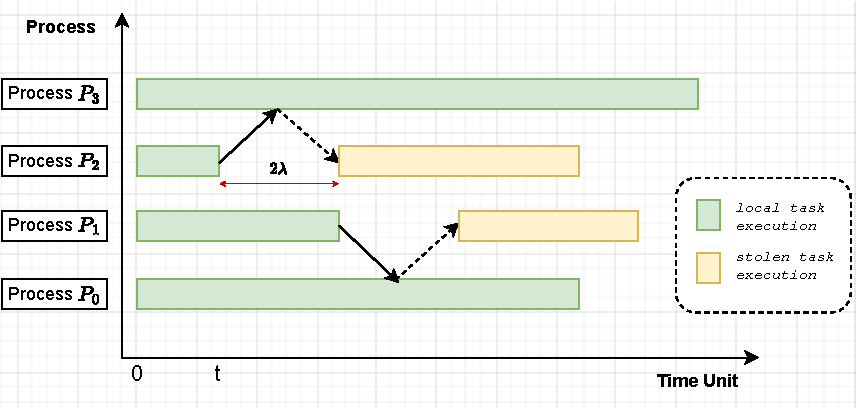
\includegraphics[scale=0.8]{./pictures/perf_analysis_model/perf_analysis_related_model_with_latency.pdf}
	\caption{An illustration of work-stealing with latency effect.}
	\label{fig:perfmodel_relatedmodelwithlatency}
\end{figure}

Figure \ref{fig:perfmodel_relatedmodelwithlatency} demonstrates a scenario of work stealing with latency. The x-axis represents the time progress of execution with four involved processes. Process $2$ is assumed idle and sends a steal request to process $3$. Since process $3$ accepts, task is sent from $3$ to $2$. We name $\lambda$ as the latency, and one stealing action takes a round-trip time $2\lambda$. This occurs similarly between process $1$ and $0$.\\

As the round-trip time of $2\lambda$ and the total amount of tasks $T$ on $P$ processes, we can drive to a straightforward bound of makespan as \ref{eq:straight_cmax}.
\begin{equation} \label{eq:straight_cmax}
\begin{split}
	P \cdot & C_{max} \leq T + 2\lambda \cdot \#{\textrm{task requests}} \\
	\Leftrightarrow \ & C_{max} \leq \frac{T}{P} + 2\lambda \cdot \frac{\#{\textrm{task requests}}}{P}
\end{split}
\end{equation}

However, to be closer to an optimal bound, this work approached a potential function bounding on the number of work-stealing requests\footnote{Work-stealing requests mean the number of requests for stealing tasks in our context. Therefore, it is also called $\#{\textrm{task requests}}$ shown in Equation \ref{eq:straight_cmax} or steal requests}. The authors reconsidered the time division as periods of duration $\lambda$ to analyze the impact of latency. To not abuse notations, we use $T_{i}(k)$ and $s_{i}(k)$ to denote the current number of tasks and the number of stolen tasks from process $i$ at time $k$; then the quantities will be $T_{i}(k\lambda)$, $s_{i}(k\lambda)$. In the interval $(\lambda (k-1), \lambda k]$, the total number of incoming work-stealing requests is defined by $r(k) = \sum_{i=1}^{\lambda} R((k-1)\lambda + i)$, where $0 \leq r(k) \geq P$. The probability, that a process receives $\geq 1$ requests in the interval $(\lambda (k-1), \lambda k]$, is $q(r(k))$.\\

Nicolas Gast et al. \cite{gast2021analysis} showed the analysis of the potential decrease, which is defined in Equation \ref{eq:potfunc_latency} at time-step $k\lambda$.
\begin{equation} \label{eq:potfunc_latency}
\begin{split}
	\Phi(k) = 1 + \frac{1}{\lambda^2} \sum_{i=1}^{P} (T_{i}(k)^2 + 2s_{i}(k)^2)
\end{split}
\end{equation}

where, $\Phi(k)$ gets through all processes $\in P$, $T_{i}(k)$ and $s_{i}(k)$ represents the number of remaining tasks as well as the number of stolen tasks in process $i$ at time $k$. Let $\Phi(0)$ be the potential at time $t_{0}$ and $\tau$ be the first time step at which the potential reaches $1$. Then, the authors proved that the number of incoming steal requests until $\tau$, $R = \sum_{k=0}^{\tau = 1} r(k)$ satisfies:
\begin{equation} \label{eq:exp_prob_R_latency}
\begin{split}
	& E[R] \leq P \gamma \log_{2} \Phi(0) \\
	& \mathbb{P}[R \leq P \gamma (\log_{2} \Phi(0) + x)] \leq 2^{-x}
\end{split}
\end{equation}

In which, $E[R]$ is the expected number of total incoming steal requests and $\mathbb{P}$ indicates the probability when $R \leq P \gamma (\log_{2} \Phi(0) + x)$, and $\gamma$ is a constant such that $\gamma < 4.03$. Applying to $C_{max}$, the study concluded as Equation \ref{eq:exp_prob_Cmax_latency} shows.

\begin{equation} \label{eq:exp_prob_Cmax_latency}
\begin{split}
	& E[C_{max}] \leq \frac{T}{P} + 4\lambda\gamma\log_{2} \frac{P}{\lambda} + 2\lambda\gamma \\
	& \mathbb{P}[C_{max} \geq \frac{T}{P} + 4\lambda\gamma\log_{2} \frac{P}{\lambda} + x] \leq 2^{\frac{-x}{2\lambda\gamma}}
\end{split}
\end{equation}


\paragraph{Further discussion:}
The mentioned models above are relevant in terms of work stealing with or without latency. However, latency $\lambda$ is a constant, and the number of steal requests must contribute relatively, such as task execution time. These constraints might be limited by the cases in that task data sizes are different or transmission time considerably impacts the efficiency of stealing operations in practice. In contrast, this thesis analyzes the performance in a different direction. We introduce a proposed model associated with transmission time or delay time. The delay happens when tasks are migrated in distributed memory. First, the delay values depend on the size of task data in movement and the current status of interconnection, e.g., latency, bandwidth. Second, we figure out that this challenge can lead to other impacts on the decision time of taking stealing or balancing actions. This is a reason causing too late to balancing load in distributed memory. Next, we will discuss about a proposed model with delay time when tasks are migrated.
